\documentclass[aspectratio=169,11pt]{beamer}

\usetheme{Madrid}
\usecolortheme{default}
\usefonttheme{professionalfonts}
\setbeamertemplate{navigation symbols}{}
\setbeamertemplate{footline}[frame number]

\usepackage{amsmath, amssymb, booktabs, graphicx}
\graphicspath{{../../assets/figures/}{assets/figures/}}

\title{Unions, Collective Bargaining, and Worker Voice}
\subtitle{Labor II --- Week 8}
\author{Teaching deck draft}
\date{}

\begin{document}

\begin{frame}
  \titlepage
\end{frame}

\begin{frame}{Central question and course repositioning}
\begin{itemize}
    \item What do unions and collective bargaining actually change in labor markets once bargaining becomes collective rather than individual?
    \item Week 8 is the institution-heavy sequel to Weeks 5--7: bargaining protocol, employer power, and wage floors now meet organized worker voice.
    \item Week 9 will then ask how labor regulation, enforcement, and insurance sustain or constrain those institutions.
\end{itemize}
\end{frame}

\begin{frame}{Week 7 to Week 8 bridge}
\begin{itemize}
    \item Week 7: legal wage floors compress pay from outside the contract.
    \item Week 8: collective bargaining can reshape wages, compression, amenities, grievance rules, and voice from inside the employment relationship.
    \item The key transition is from decentralized wage rules to organized worker bargaining power.
\end{itemize}
\end{frame}

\begin{frame}{What unions and collective bargaining change}
\begin{itemize}
    \item Wage levels and rent-sharing.
    \item Wage structure and compression.
    \item Benefits, schedules, and job protection.
    \item Grievance procedures and worker voice.
    \item Employer behavior through threat effects and organizing avoidance.
\end{itemize}
\[
w_{ijt} = w^0_{ijt} + \beta_{jt} R_{jt}
\]
\end{frame}

\begin{frame}{Membership versus coverage versus bargaining regime}
\begin{center}
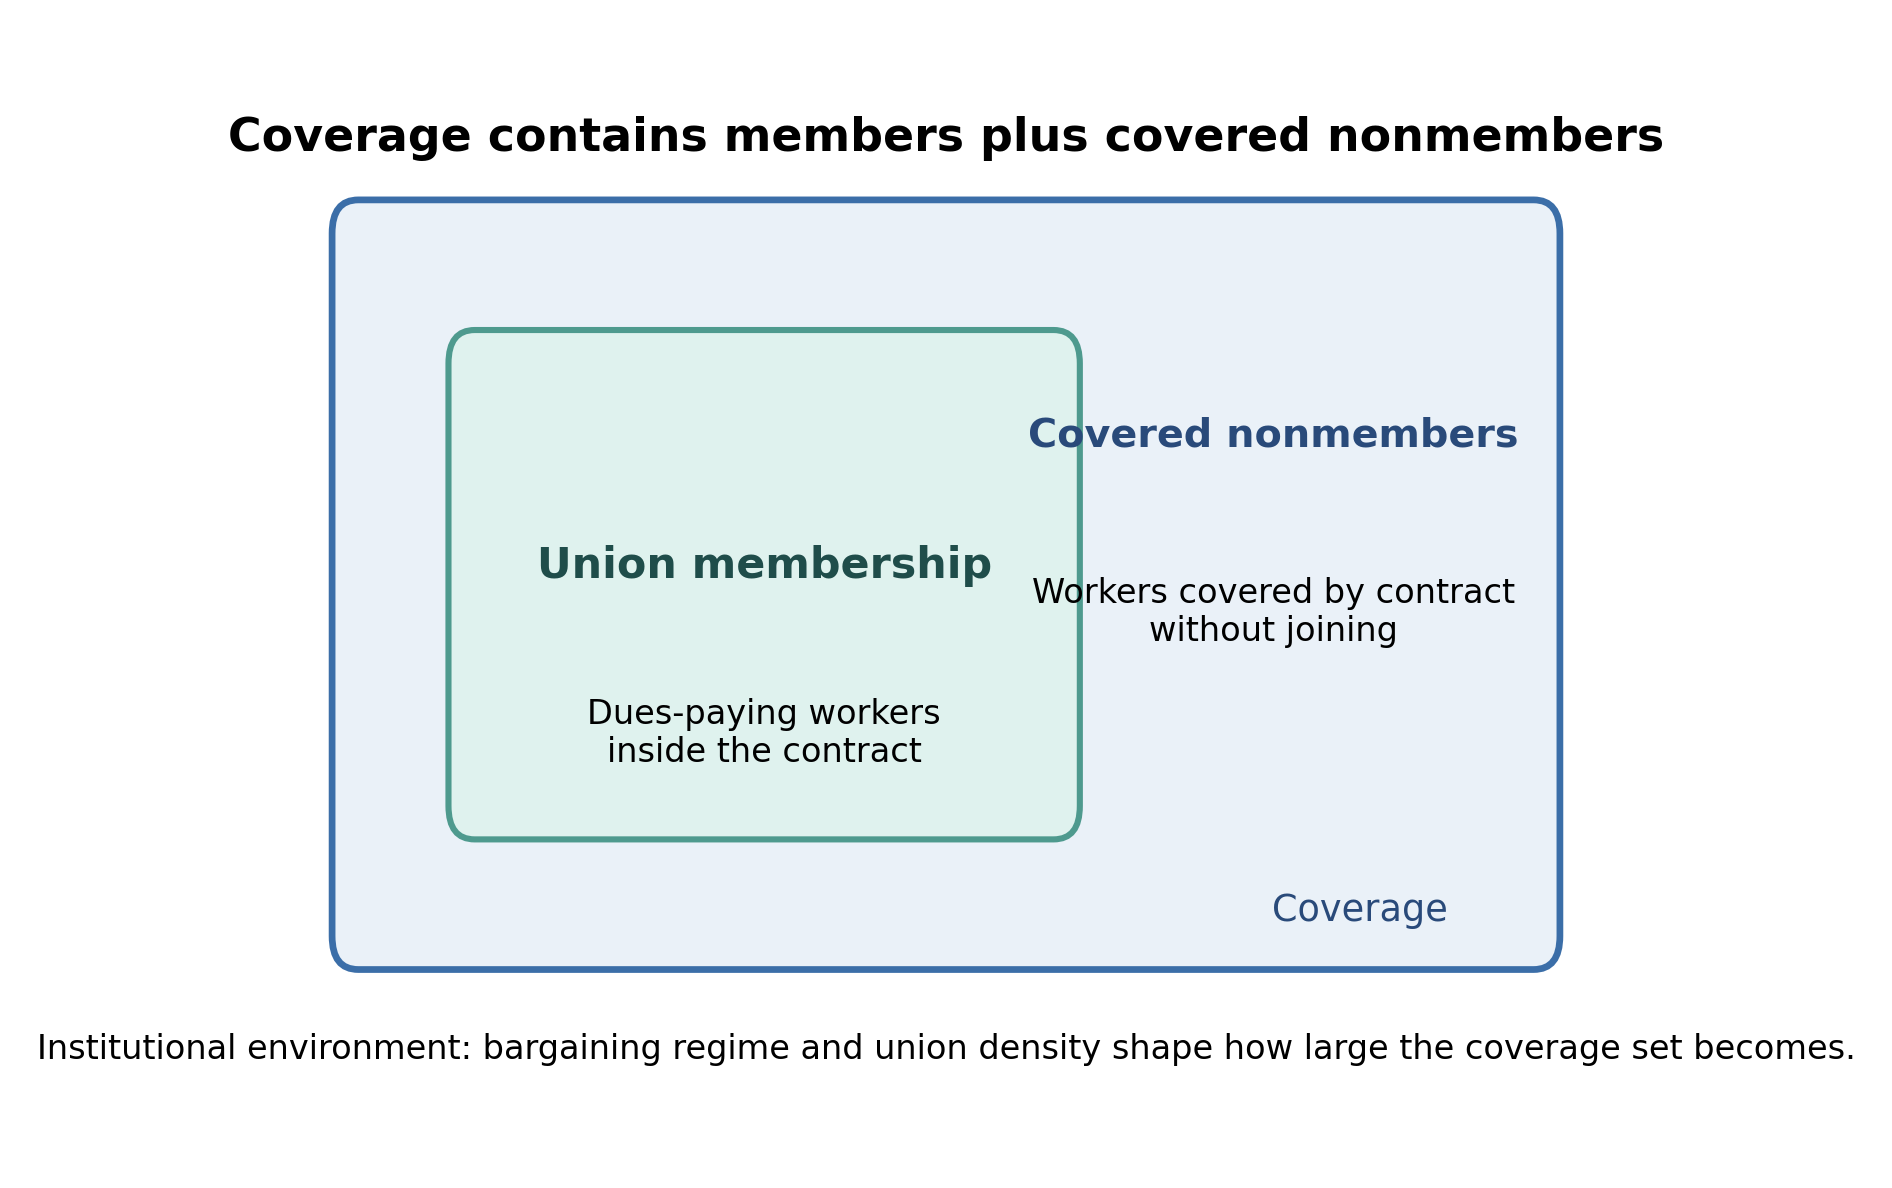
\includegraphics[height=0.72\textheight]{08-membership-vs-coverage-distinction.png}
\end{center}
\end{frame}

\begin{frame}{Coverage is not membership}
\[
C_{rt} = M_{rt} + N^{covered,nonmember}_{rt},
\qquad
C_{rt} \geq M_{rt}
\]

\begin{itemize}
    \item Membership is organizational attachment.
    \item Coverage is the contract object.
    \item Density is the surrounding environment for spillovers and politics.
    \item Regime tells us whether bargaining is firm-level, sectoral, multi-employer, or extended.
\end{itemize}
\end{frame}

\begin{frame}{Bargaining regimes}
\begin{center}
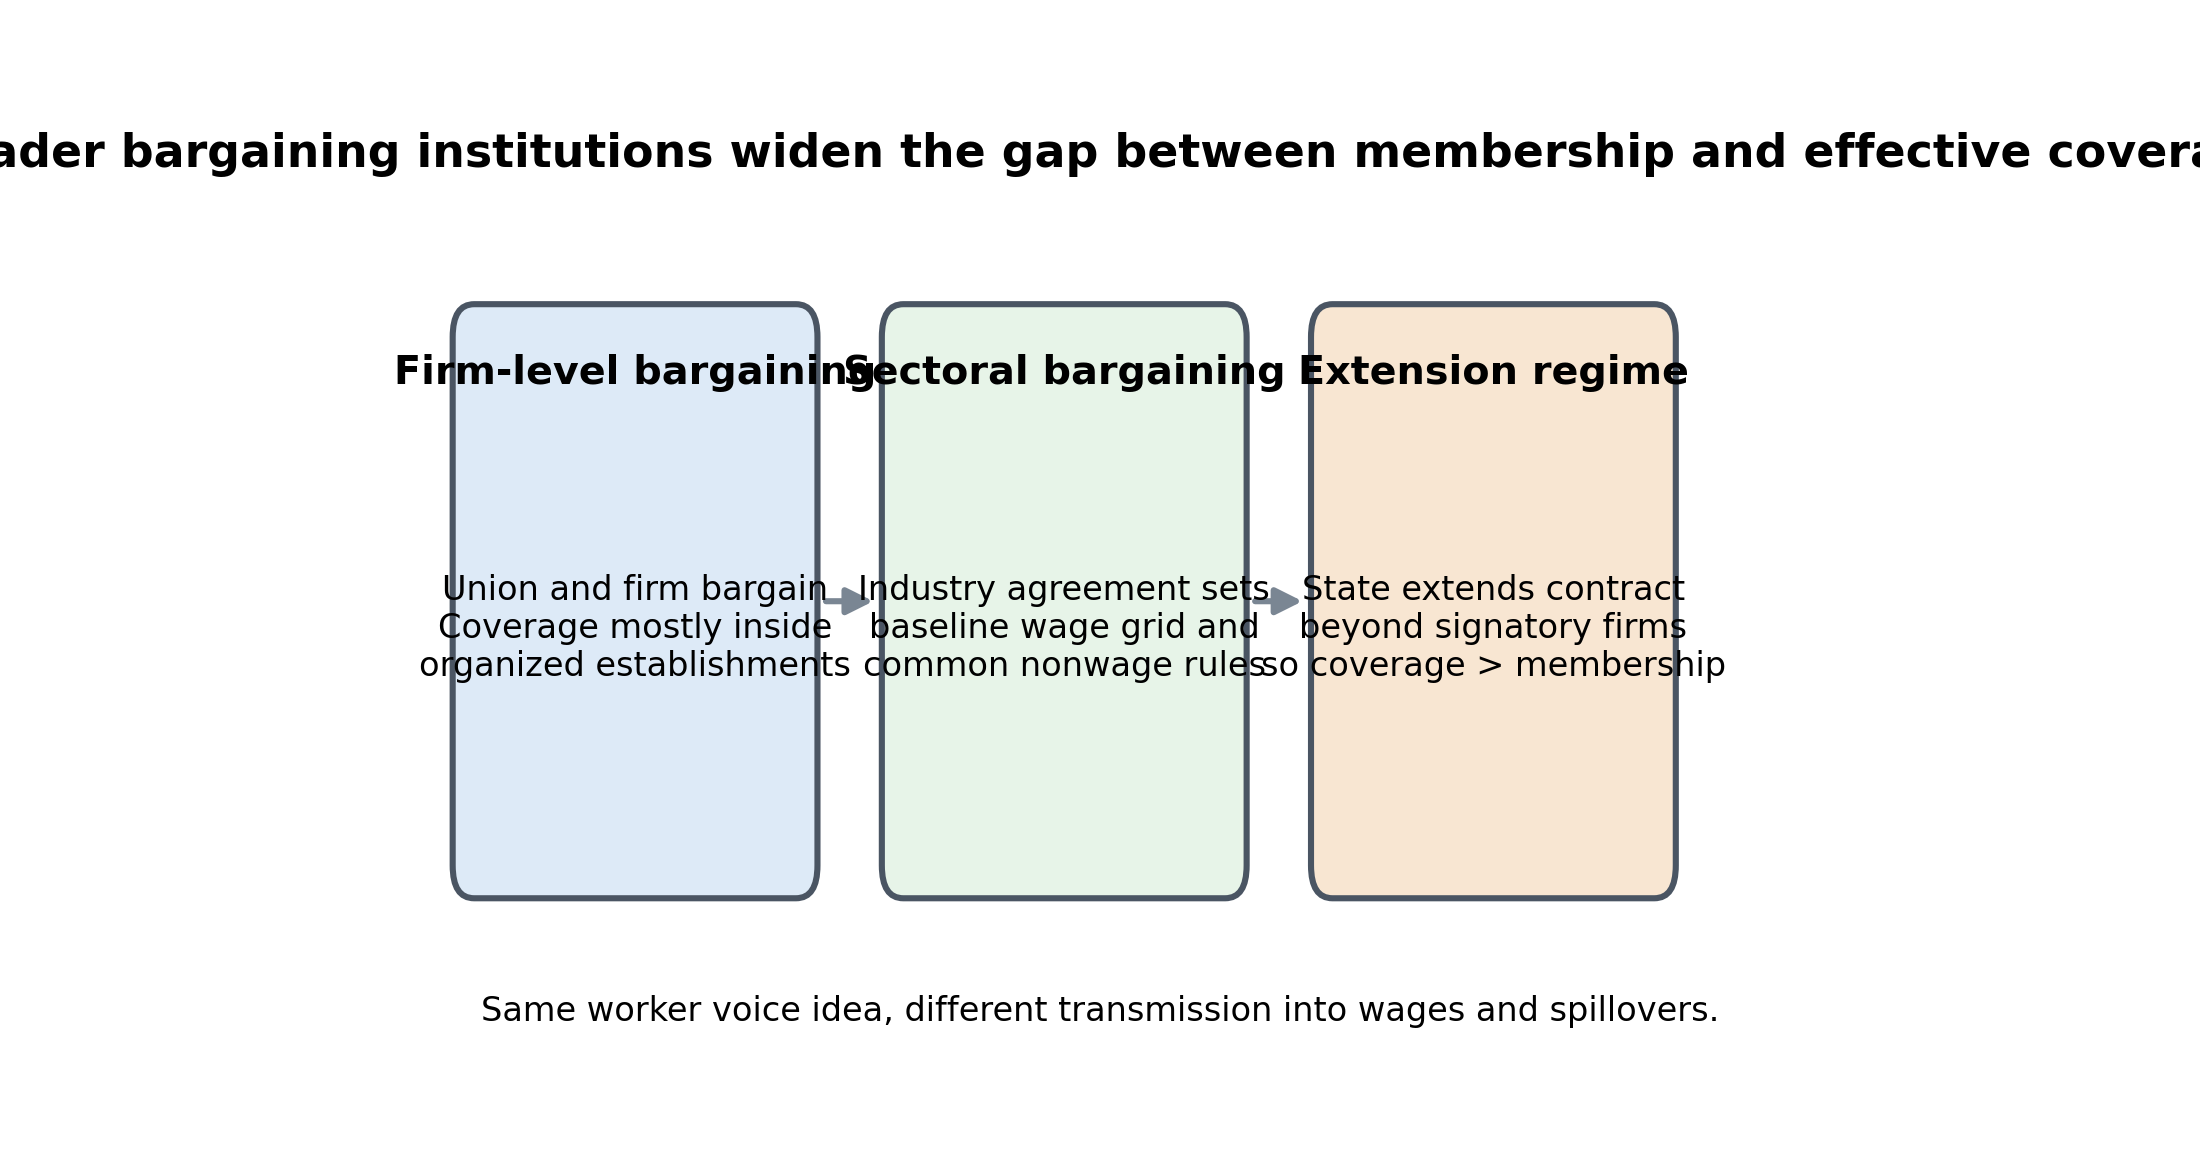
\includegraphics[height=0.72\textheight]{08-collective-bargaining-regimes.png}
\end{center}
\end{frame}

\begin{frame}{Union takeup, organizing, and certification}
\[
\Pr(\text{UnionWin}_{jt}=1) = F(D_{jt}, O_{jt}, L_{jt})
\]

\begin{itemize}
    \item Worker demand is not the same thing as realized unionization.
    \item Organizing depends on employer opposition, legal rules, and local labor-market conditions.
    \item Certification elections are central in the U.S. private-sector literature because they generate close-win variation.
    \item Organizing success is an entry point into coverage, not the same thing as equilibrium union density.
\end{itemize}
\end{frame}

\begin{frame}{From worker demand to realized coverage}
\begin{center}
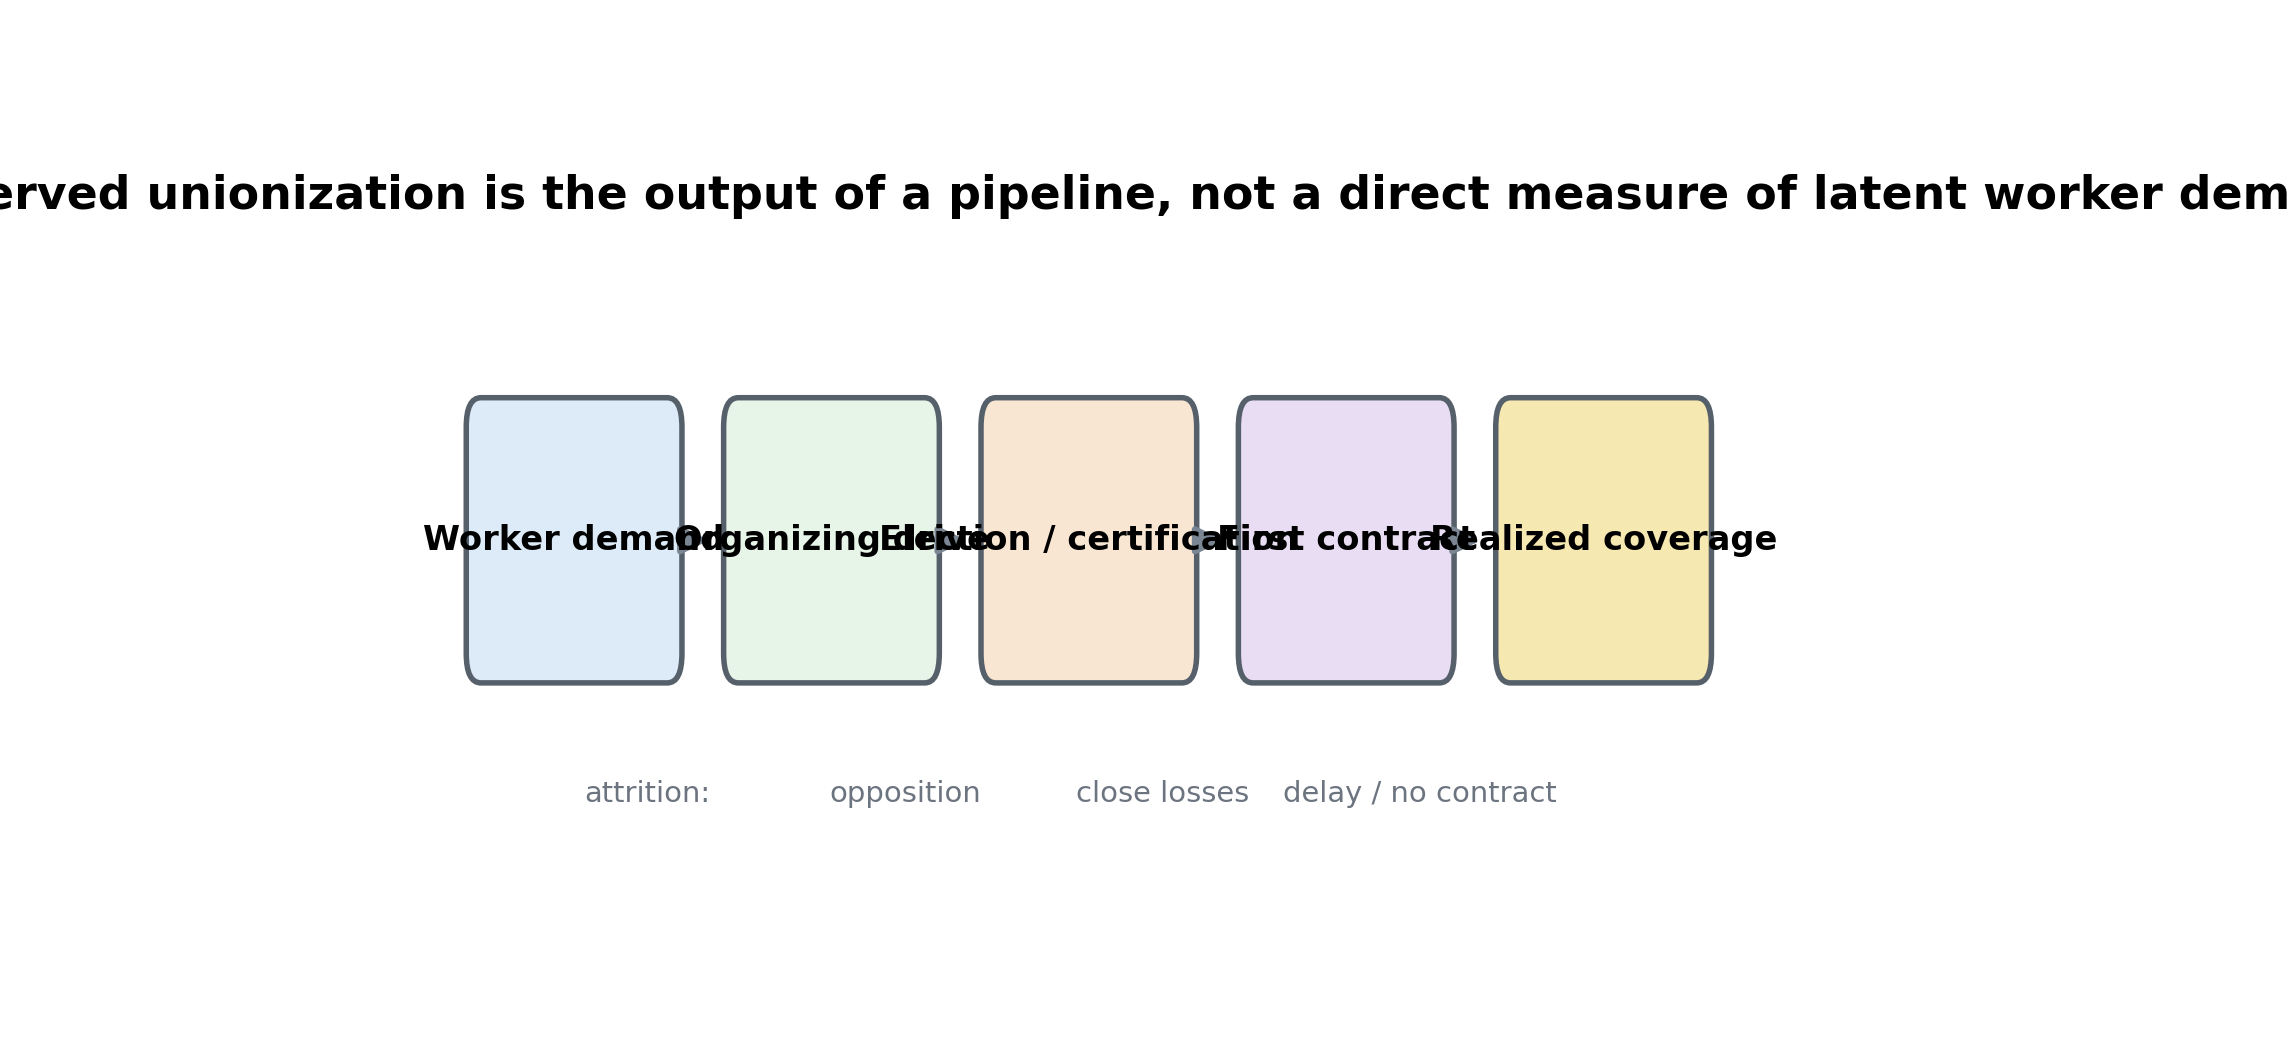
\includegraphics[height=0.72\textheight]{08-certification-to-coverage-pipeline.png}
\end{center}
\end{frame}

\begin{frame}{Direct effects on covered workers}
\begin{itemize}
    \item Distinguish union wage premia from broader coverage premia.
    \item DiNardo-Lee: close-election RD identifies a local effect of marginal union wins on establishments.
    \item Frandsen: matched employer-employee data reveal payroll, earnings, and composition effects more directly.
    \item Farber-Herbst-Kuziemko-Naidu: unions matter for wage compression and inequality over time, not only for a point premium.
\end{itemize}
\end{frame}

\begin{frame}{Compression, spillovers, and threat effects}
\[
w^N_{rt} = \alpha + \gamma \,\text{UnionPresence}_{rt} + X'_{rt}\delta + \varepsilon_{rt}
\]

\begin{itemize}
    \item Direct effects on covered workers are not the whole story.
    \item Spillovers can be positive, negative, or threat-based.
    \item Nonunion workers inside unionized firms are often contaminated controls.
    \item Aggregate inequality effects depend on uncovered workers too.
\end{itemize}
\end{frame}

\begin{frame}{Wage compression and spillovers}
\begin{center}
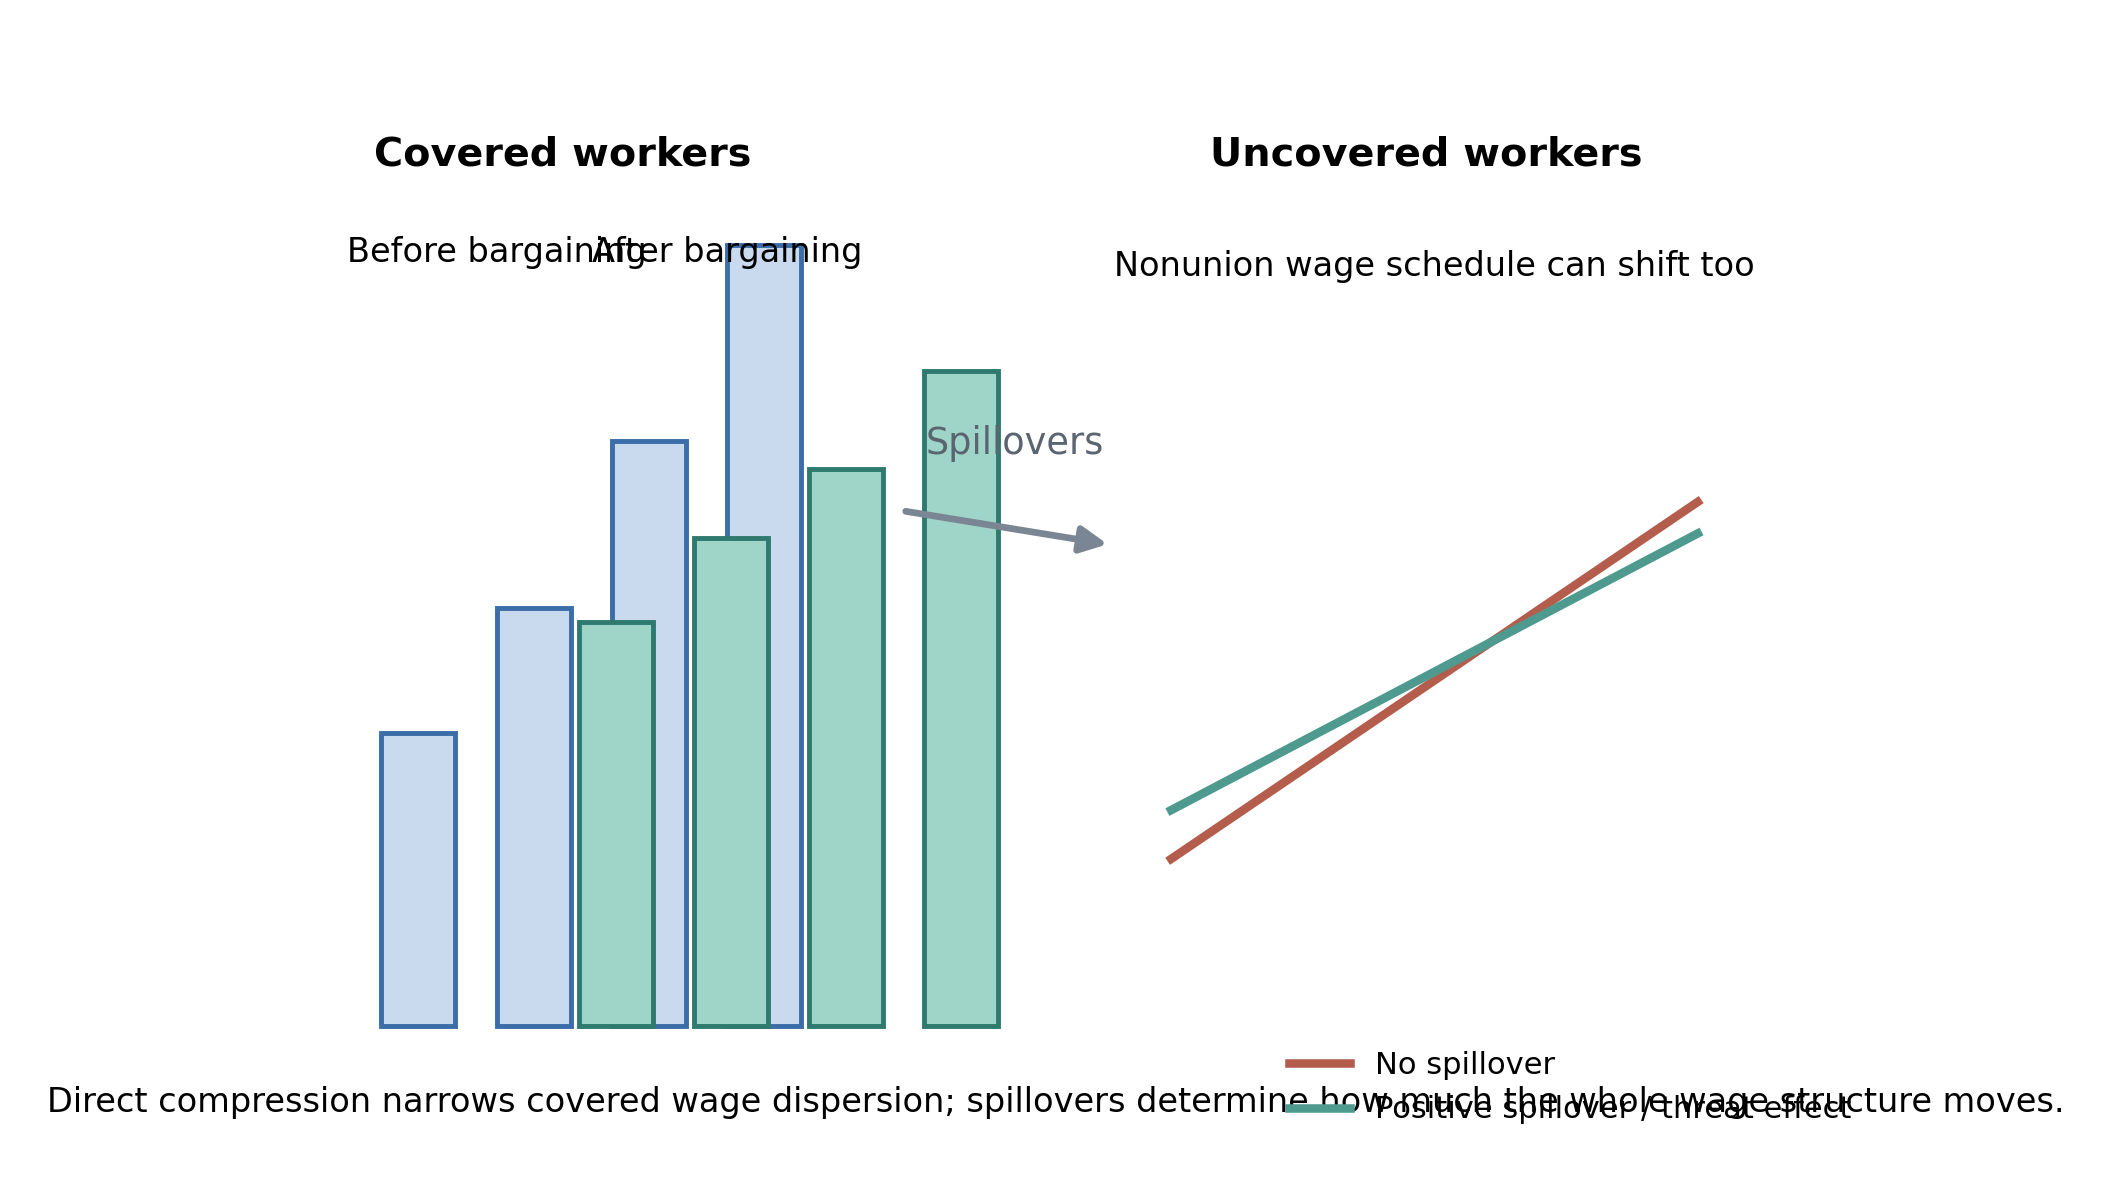
\includegraphics[height=0.72\textheight]{08-union-wage-compression-and-spillovers.png}
\end{center}
\end{frame}

\begin{frame}{Empirical designs and what they identify}
\small
\begin{tabular}{p{0.19\linewidth} p{0.2\linewidth} p{0.18\linewidth} p{0.3\linewidth}}
\toprule
Design & Unit & Best object & Main limitation \\
\midrule
Close-election RD & Establishment / election & Local effect of union victory & Local treatment effect only \\
Matched worker-firm & Worker-firm match & Earnings, payroll, composition & Restricted data; spillovers remain \\
Historical decomposition & Worker-year / state-year & Wage compression, inequality & Stronger assumptions \\
Cross-country coverage & Worker-country-year & Regime and coverage effects & Institutions move jointly \\
Policy-shock event study & State-year / sector-year & Law and bargaining-rule changes & Policy endogeneity \\
\bottomrule
\end{tabular}
\end{frame}

\begin{frame}{Political-economy bridge}
\begin{center}
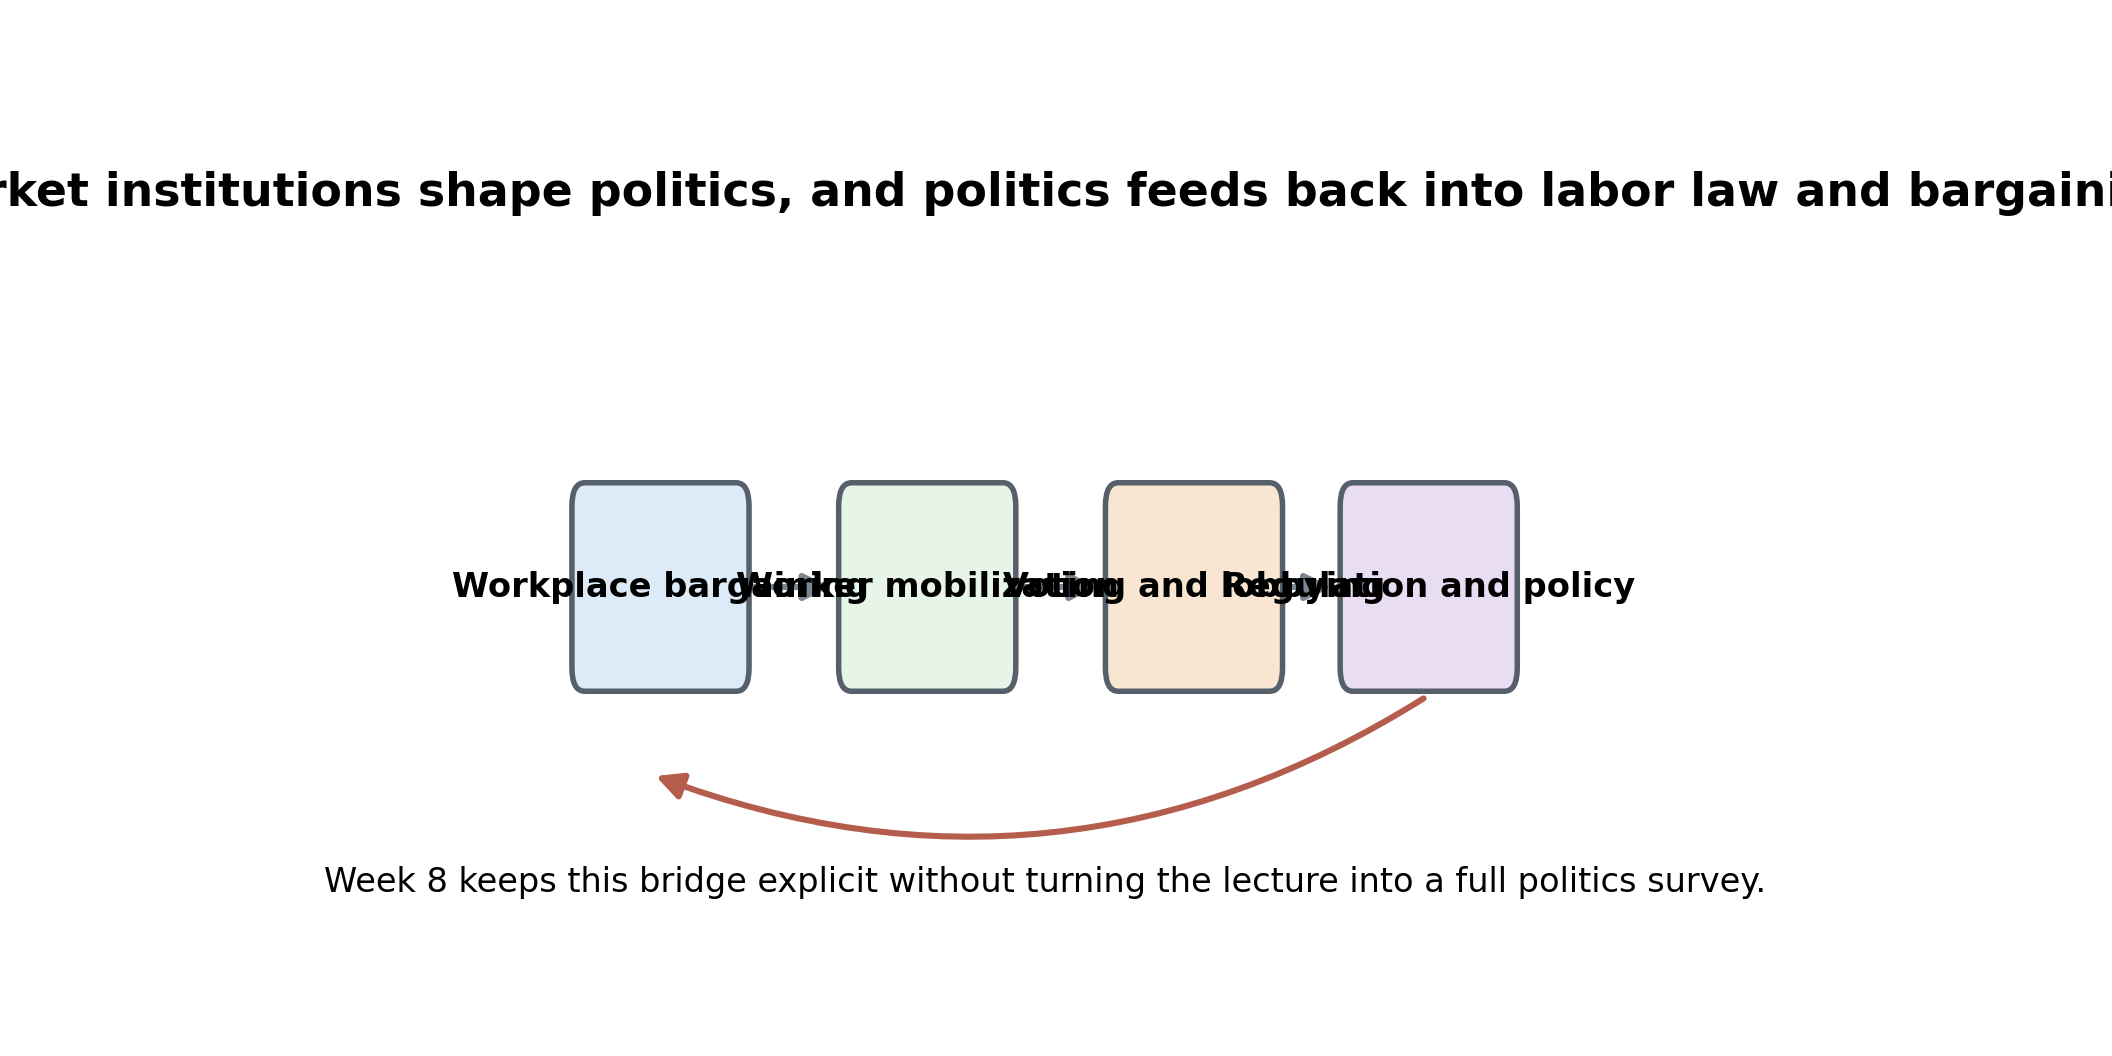
\includegraphics[height=0.66\textheight]{08-political-economy-bridge.png}
\end{center}
\begin{itemize}
    \item Unions are labor-market institutions and political actors.
    \item Politics matters here because it feeds back into labor law, enforcement, and insurance.
    \item The main estimands this week still remain wages, employment, coverage, and spillovers.
\end{itemize}
\end{frame}

\begin{frame}{Frontier extension block}
\begin{itemize}
    \item Coverage regimes and international heterogeneity.
    \item Unions as a counterweight to monopsony.
    \item Within-firm spillovers for uncovered workers.
    \item New data on campaigns, elections, and worker beliefs.
    \item Organizing under tight labor markets, automation, and remote work.
\end{itemize}
\end{frame}

\begin{frame}{Bridge to Week 9}
\begin{itemize}
    \item Week 8 introduced bargaining institutions, worker voice, and organizing.
    \item Week 9 asks how labor regulation, enforcement, and insurance change the legal environment in which those institutions operate.
    \item The transition question is how bargaining power interacts with regulation, compliance, and public protection.
\end{itemize}
\end{frame}

\begin{frame}{Takeaways}
\begin{itemize}
    \item Membership, coverage, bargaining regime, and worker voice are different objects.
    \item Organizing and certification are not the same thing as post-union wage or employment effects.
    \item Direct effects on covered workers and spillovers onto uncovered workers must be kept separate.
    \item Unions matter for labor economics because they change wage-setting, inequality, and the institutional environment around work.
\end{itemize}
\end{frame}

\appendix

\begin{frame}{Appendix: lab bridge}
\begin{itemize}
    \item Reproduce: a Farber-Herbst-Kuziemko-Naidu style synthetic coverage-and-inequality panel.
    \item Diagnose: a DiNardo-Lee style synthetic close-election RD.
    \item Transfer: CPS/Unionstats coverage panels, certification-election panels, or a spillover design inspired by Fortin-Lemieux-Lloyd.
    \item Keep the object straight: membership, coverage, organizing margin, direct effect, or spillover effect.
\end{itemize}
\end{frame}

\end{document}
